%  Trustworthy Drug Repurposing Recommendation via Knowledge-Graph-Grounded LLMs
%  MDPI Electronics, special issue "Recommendation Systems: Recent Advances and Future Directions"
%  Build:  cd paper && pdflatex main && bibtex main && pdflatex main && pdflatex main
%  Numbers: experiments/make_results.py -> results/tables/results.json and paper/tables/*.tex
%  \TODO{...} marks text that still needs a result or an author decision.
\documentclass[electronics,article,submit]{Definitions/mdpi}

\usepackage{iftex}
\ifXeTeX  % local preview build with tectonic only: no Ghostscript for the EPS logos, use stubs
  \makeatletter\let\mdpi@orig@includegraphics\includegraphics
  \renewcommand{\includegraphics}[2][]{\def\mdpi@f{#2}\def\mdpi@a{Definitions/logo-mdpi.eps}\def\mdpi@b{Definitions/logo-updates.eps}%
    \ifx\mdpi@f\mdpi@a\mdpi@orig@includegraphics[#1]{build_stub/logo-mdpi.pdf}%
    \else\ifx\mdpi@f\mdpi@b\mdpi@orig@includegraphics[#1]{build_stub/logo-updates.pdf}%
    \else\mdpi@orig@includegraphics[#1]{#2}\fi\fi}\makeatother
\fi
\usepackage{xurl}  % break long URLs (repository link)
\usepackage{tikz}
\usetikzlibrary{arrows.meta,positioning,fit}
\newcommand{\TODO}[1]{\textcolor{red}{[TODO: #1]}}
\newcommand{\dmrr}{$\Delta$MRR}
\makeatletter\newcommand{\tabinput}[1]{\@@input #1 }\makeatother  % \input is not expandable inside tabular

\firstpage{1}
\makeatletter
\setcounter{page}{\@firstpage}
\makeatother
\pubvolume{1}
\issuenum{1}
\articlenumber{0}
\pubyear{2027}
\copyrightyear{2027}
\datereceived{ }
\daterevised{ }
\dateaccepted{ }
\datepublished{ }
\hreflink{https://doi.org/}

\Title{Trustworthy Drug Repurposing Recommendation via Knowledge-Graph-Grounded Large Language Models}
\TitleCitation{Trustworthy Drug Repurposing Recommendation via Knowledge-Graph-Grounded Large Language Models}
\Author{Kallol Naha $^{1}$ and Hasan Jamil $^{1,}$*}
\AuthorNames{Kallol Naha and Hasan Jamil}
\AuthorCitation{Naha, K.; Jamil, H.}
\address{$^{1}$ \quad Department of Computer Science, University of Idaho, 875 Perimeter Dr, Moscow, ID 83844, USA; naha7197@vandals.uidaho.edu}
\corres{Correspondence: jamil@uidaho.edu}

\abstract{Drug repurposing can be framed as a recommendation problem: for each disease, rank existing drugs by how likely they are to treat it. Knowledge-graph (KG) embedding models give useful rankings but no reasons, while large language models (LLMs) give fluent reasons that may be invented. We study a two-stage recommender that keeps the two roles apart. A RotatE model trained on PrimeKG proposes the top-20 drugs for each disease; for each candidate we retrieve up to ten 2--3-hop KG paths, and an LLM must explain the candidate using only those paths, cite them, and return a confidence that re-ranks the list. Every recommendation is logged with full provenance. On 939 held-out indications, grounded re-ranking raises MRR from 0.179 to 0.247--0.264 for four of five LLMs, and the paths add 0.03--0.05 MRR over the same LLMs without paths. Cited claims are almost always supported by the cited paths (97--99\%), but free-text mechanisms are not (14--28\% supported); requiring every mechanism sentence to cite paths raises this to 88--91\% at a small cost in accuracy. Raw confidences are badly over-confident (ECE 0.24--0.29) yet rank well (AUROC 0.80--0.90), and a two-parameter Platt map fitted on validation diseases reduces ECE to below 0.015. Grounding is also a vulnerability: three fake KG chains per decoy drug lift it to the top rank for up to 20\% of diseases, and the LLM cites the fake edges in over 98\% of those explanations. On 136 diseases whose drug edges are all withheld from training, grounded re-ranking raises MRR from 0.109 to 0.148--0.190, the paths add 0.03--0.05 MRR for four of five LLMs, and the gain comes almost entirely from paths through indications of ontologically related diseases; TxGNN, designed for this setting, reaches MRR 0.040 in our protocol.}

\keyword{drug repurposing; recommender systems; knowledge graphs; large language models; retrieval-augmented generation; explainability; faithfulness; calibration; data poisoning; provenance}

\begin{document}

%======================================================================
\section{Introduction}
%======================================================================
Developing a new drug takes more than a decade and fails far more often than it succeeds; finding new uses for approved drugs, or \emph{drug repurposing}, reuses known safety profiles and can shorten that path considerably~\cite{pushpakom2019}. Computationally, repurposing is a recommendation problem: the \emph{users} are diseases, the \emph{items} are drugs, and the observed interactions are known indications. Biomedical knowledge graphs (KGs) such as Hetionet~\cite{himmelstein2017hetionet} and PrimeKG~\cite{chandak2023primekg} supply the side information that links drugs to diseases through targets, pathways and phenotypes, and KG link-prediction models rank candidate drugs for a disease from that structure~\cite{bordes2013transe,sun2019rotate,huang2024txgnn}.

A ranked list is not enough for this domain. A clinician or pharmacologist who acts on a recommendation needs to know \emph{why} a drug is suggested, how much to trust the suggestion, and where the evidence came from. Embedding-based rankers provide none of this. Large language models (LLMs) can write convincing explanations and have been adopted widely as recommenders and re-rankers~\cite{wu2024llmrec}, but their explanations may contain facts that appear nowhere in the evidence~\cite{ji2023hallucination}, and their stated confidences are often poorly calibrated~\cite{kadavath2022know,xiong2024uncertainty}. Retrieval-augmented generation~\cite{lewis2020rag} and KG grounding~\cite{pan2024unifying} are the standard answers to hallucination, but grounding moves trust onto the graph: if the graph contains wrong or planted edges, a grounded model may faithfully explain a false recommendation.

This paper studies a recommender that separates the roles explicitly. A KG embedding model (RotatE~\cite{sun2019rotate}) generates candidates; for each disease--drug pair we retrieve 2--3-hop paths from the training graph; an LLM must explain the pair \emph{using only those paths}, cite the paths behind every claim, and output a confidence that re-ranks the candidates. Each recommendation is stored with its data version, model checkpoint, prompt, retrieved paths and raw response. We then measure the properties that make such a recommender trustworthy, not only accurate:
\begin{itemize}
\item \textbf{Accuracy.} Does grounded LLM re-ranking improve on the KG model and on the same LLM without paths? We compare five open-weight LLMs from four families and report disease-level bootstrap confidence intervals, three training seeds for RotatE, and the TxGNN foundation model~\cite{huang2024txgnn} as an external baseline.
\item \textbf{Faithfulness.} Are the explanations supported by the retrieved paths? We separate cited claims from free-text mechanism sentences, and test a prompt that forces every sentence to cite paths.
\item \textbf{Calibration.} Do confidences mean what they say, and can a map fitted on validation diseases repair them?
\item \textbf{Robustness.} What happens when the graph is poisoned, at training time and at retrieval time?
\end{itemize}

Our findings are mixed in a useful way. Grounded re-ranking improves accuracy for four of the five LLMs, and part of the gain comes from the paths rather than from the LLM's prior knowledge. Citation-level faithfulness is near perfect, but the free-text mechanism is mostly not supported by the paths until citations are required. Confidences rank well but are badly over-confident, which simple post-hoc recalibration fixes. Finally, the same grounding that makes explanations verifiable lets a few planted edges promote a decoy drug, with an explanation that cites the planted edges. We release the code, prompts and provenance logs at \url{https://github.com/utpoln/trustworthy-drug-repurposing}.

%======================================================================
\section{Related Work}
%======================================================================
\textbf{KG-based drug repurposing.} Hetionet~\cite{himmelstein2017hetionet} showed that drug--disease edges can be predicted from integrated heterogeneous networks using degree-weighted path counts. Graph neural networks model polypharmacy and drug--target structure~\cite{zitnik2018decagon}. PrimeKG~\cite{chandak2023primekg} integrates twenty resources into a precision-medicine KG with indication, contraindication and off-label edges, and TxGNN~\cite{huang2024txgnn} trains a graph foundation model on it, with a metric-learning module for diseases that have no known treatments and a path-based explainer evaluated with clinicians. Translational and rotational embeddings such as TransE~\cite{bordes2013transe} and RotatE~\cite{sun2019rotate}, available in PyKEEN~\cite{ali2021pykeen}, remain strong general-purpose link predictors.

\textbf{Knowledge-aware and explainable recommendation.} KGs have long been used to make recommendations both more accurate and more explainable, e.g. by attention over KG neighbourhoods~\cite{wang2019kgat}; see~\cite{zhang2020explainable} for a survey of explainable recommendation. LLMs are now used as recommenders, re-rankers and explanation generators~\cite{wu2024llmrec}. Our setting is a two-stage recommender in this line, where the explanation is constrained to KG evidence and checked against it.

\textbf{Grounding, faithfulness and LLM judges.} Retrieval-augmented generation conditions an LLM on retrieved evidence~\cite{lewis2020rag}, and KG--LLM integration is an active area~\cite{pan2024unifying}. Faithfulness of generated text to its evidence is typically scored by decomposing the output into statements and checking each against the context, often with an LLM as judge~\cite{es2024ragas,zheng2023judge}. We follow this approach and validate the judge against human labels.

\textbf{Calibration.} Expected calibration error (ECE)~\cite{naeini2015ece} and post-hoc maps such as temperature scaling~\cite{guo2017calibration}, Platt scaling~\cite{platt1999} and isotonic regression~\cite{zadrozny2002} are standard for classifiers. LLMs can express useful uncertainty but tend to be over-confident when asked verbally~\cite{kadavath2022know,xiong2024uncertainty}.

\textbf{Poisoning.} Small, targeted perturbations of graph data can change the predictions of graph neural networks~\cite{zugner2018nettack} and KG embeddings~\cite{zhang2019kgepoison}. We extend this concern to grounded LLMs, where poisoned edges can enter both the candidate generator and the evidence that the LLM explains.

%======================================================================
\section{Materials and Methods}
%======================================================================
\begin{figure}[H]
\centering
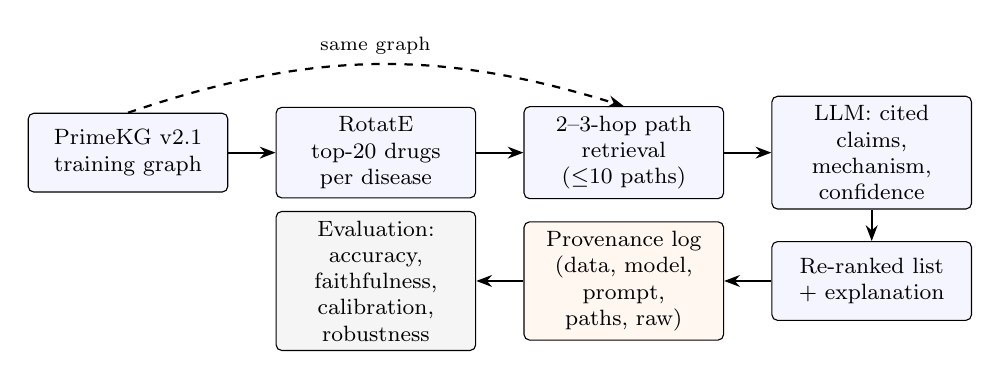
\begin{tikzpicture}[node distance=4mm and 6mm, font=\footnotesize,
  box/.style={draw, rounded corners=2pt, align=center, minimum height=10mm, text width=23mm, fill=blue!4},
  arr/.style={-{Stealth[length=2mm]}, thick}]
\node[box] (kg) {PrimeKG v2.1\\training graph};
\node[box, right=of kg] (kge) {RotatE\\top-20 drugs\\per disease};
\node[box, right=of kge] (ret) {2--3-hop path\\retrieval\\(${\le}$10 paths)};
\node[box, right=of ret] (llm) {LLM: cited claims,\\mechanism,\\confidence};
\node[box, below=of llm] (rank) {Re-ranked list\\+ explanation};
\node[box, left=of rank, fill=orange!6] (prov) {Provenance log\\(data, model,\\prompt, paths, raw)};
\node[box, left=of prov, fill=gray!8] (eval) {Evaluation: accuracy,\\faithfulness, calibration,\\robustness};
\draw[arr] (kg) -- (kge); \draw[arr] (kge) -- (ret); \draw[arr] (ret) -- (llm); \draw[arr] (llm) -- (rank);
\draw[arr] (rank) -- (prov); \draw[arr] (prov) -- (eval);
\draw[arr, dashed] (kg.north) to[bend left=18] node[above, font=\scriptsize] {same graph} (ret.north);
\end{tikzpicture}
\caption{Pipeline. The candidate generator and the path retriever use the same training graph, from which all held-out indications have been removed. The LLM sees only the retrieved paths (grounded mode) or only the names (no-paths baseline).\label{fig:pipeline}}
\end{figure}

\subsection{Data and Splits}
We use PrimeKG v2.1~\cite{chandak2023primekg} (129,375 nodes; 30 relation types). PrimeKG lists each edge in both directions; we keep one canonical direction per edge, giving 4,050,064 triples. The recommendation targets are the 9,388 unique drug--disease \texttt{indication} pairs, split at random (seed 42) into 7,510 / 939 / 939 train / validation / test pairs; the test set covers 496 diseases and 586 drugs. For every held-out pair we also remove any \texttt{contraindication} or \texttt{off-label use} edge between the same drug and disease from the training graph (50 edges), since those edges would reveal the answer. The training graph (4,048,136 triples) is the only graph seen by the candidate generator and by the retriever.

We additionally build a \emph{disease-held-out} split for the zero-shot repurposing setting~\cite{huang2024txgnn}: 10\% of diseases with at least one indication are assigned to test and 10\% to validation, and \emph{all} drug--disease edges of those diseases (indications, contraindications and off-label uses) are removed from training, while their gene, phenotype and ontology edges remain. This yields 876 test indications over 136 diseases and 947 validation indications over 137 diseases.

\subsection{Candidate Generation}
We train RotatE~\cite{sun2019rotate} and TransE~\cite{bordes2013transe} with PyKEEN~\cite{ali2021pykeen} on the full training graph (embedding dimension 256, 16 negatives per positive, batch size 8,192, learning rate $10^{-3}$, up to 50 epochs with early stopping on validation MRR). Candidates for disease $s$ are all 7,957 drug nodes, scored as tails of $(d,\texttt{indication},s)$. Following the filtered protocol, other known indications of $s$ (from any split) are removed before ranking a target, and ties are resolved with the realistic (mean) rank. RotatE is trained with three seeds (42, 1, 2) to measure training variance; the LLM experiments use the seed-42 candidates.

As an external baseline we train TxGNN~\cite{huang2024txgnn} (official code, commit \texttt{0e0203c}) on exactly our training graph, using the published defaults (hidden size 100, three prototypes, all-nodes-profile similarity, rarity aggregation; pre-training 2 epochs at learning rate $10^{-3}$, fine-tuning 500 epochs at $5\times10^{-4}$). For CPU feasibility, we increase the pre-training batch size from 1,024 to 4,096. TxGNN scores are ranked with the same filtered protocol.

\subsection{Path Retrieval}
For each test disease we take the top $k=20$ RotatE candidates. For each disease--drug pair we enumerate all 2- and 3-hop paths from the drug to the disease in the training graph, restricted to mechanism-related relations (drug--protein, protein--protein, disease--protein, drug and disease phenotype relations, pathway membership and a small set of ontology edges); direct drug--disease edges are excluded. Paths are ranked by the degree-weighted path score of Hetionet~\cite{himmelstein2017hetionet}, $w(p)=\prod_{v\in p^{\circ}} \deg(v)^{-0.5}$ over intermediate nodes $p^{\circ}$, so paths through hubs are down-weighted. The ten highest-weighted paths are verbalised (e.g.\ \textit{drug --[target]$\to$ GENE --[associated with]$\to$ disease}) and numbered P1--P10.

\subsection{Grounded Explanation and Re-Ranking}
Each pair is sent to the LLM with a system prompt (Appendix~\ref{app:prompts}) that requires it to (i) use only the given paths, (ii) give a list of claims, each citing the path IDs that state it, (iii) write a short mechanism built from the claims, and (iv) output a confidence in $[0,1]$ that the drug is an effective treatment. The response must be a single JSON object. In the \emph{no-paths} baseline the same LLM receives only the disease and drug names and returns a mechanism and a confidence. All calls use temperature 0 and a 4,096-token limit; reasoning traces are discarded before parsing. Candidates are re-ranked by confidence, with ties broken by the RotatE rank; unparsable responses get confidence 0. We also report reciprocal rank fusion (RRF, $k=60$)~\cite{cormack2009rrf} of the RotatE and LLM rankings. Because only the top 20 are re-ranked, gold drugs outside the top 20 keep their RotatE rank; 37.7\% of test pairs have the gold drug inside the top 20, which bounds what re-ranking can achieve.

We compare five open-weight LLMs served through the University of Idaho MindRouter gateway~\cite{sheneman2026mindrouter}, an OpenAI-compatible vLLM endpoint: Qwen3.8-27B (dense)~\cite{qwen2026qwen38}, Gemma-4-31B (dense)~\cite{gemma2026gemma4}, Qwen3.5-122B (mixture-of-experts, MoE)~\cite{qwen2026qwen35}, gpt-oss-120B (MoE)~\cite{openai2025gptoss} and Kimi-K3 (MoE, the largest)~\cite{kimi2026k3}. This set spans four model families, dense and MoE designs, and a within-family size comparison (Qwen3.8-27B vs.\ Qwen3.5-122B).

\subsection{Provenance}
Every LLM call writes one JSON record containing: the PrimeKG release and file hash, the split directory, the KG model run and checkpoint, the LLM identifier, the prompt template version and full prompt text, the retrieved paths with their weights, the raw response (including any reasoning text), the parsed output, latency, token counts and a UTC timestamp. All tables in this paper are regenerated from these records by a single script.

\subsection{Evaluation}
\textbf{Accuracy.} We report MRR and Hits@\{1,3,10\} over the 939 test pairs. Differences between methods are given with 95\% percentile confidence intervals from a paired cluster bootstrap over test diseases (2,000 resamples)~\cite{efron1993bootstrap}, so that pairs of the same disease are resampled together.

\textbf{Faithfulness.} For 100 test diseases sampled at random (2,000 pairs per model) we split each explanation into statements: each cited claim, and each sentence of the mechanism. A judge LLM outside the compared set (Nemotron-3-Super-120B~\cite{nvidia2026nemotron3super}) labels every statement \textsc{supported}, \textsc{partial} or \textsc{unsupported} given the paths---only the cited paths for cited statements, any path otherwise---and is told not to use outside knowledge (Appendix~\ref{app:prompts}). We also check that every cited ID exists. To validate the judge, the first author labelled a stratified sample of 126 statements (three models $\times$ \{claim, mechanism\} $\times$ three judge labels) without seeing the judge's labels; we report agreement as Cohen's $\kappa$~\cite{cohen1960kappa}. \TODO{human-label results; if the labels start from the AI-drafted sheet, say so here (``labels drafted by an AI assistant and checked by the first author'').}

A second prompt (v2) replaces the free-text mechanism with a list of sentences, each of which must cite the paths it restates, or state that the paths do not establish a mechanism. We run v2 with Qwen3.8-27B and Gemma-4-31B on the same 100 diseases.

\textbf{Calibration.} We compute ECE with ten equal-width bins~\cite{naeini2015ece}, the Brier score and AUROC over all disease--candidate pairs, where the label is whether the candidate is a held-out indication (base rate 3.5\%). To test post-hoc repair, we run every model in grounded mode on 100 validation diseases (2,000 pairs), fit temperature scaling~\cite{guo2017calibration}, Platt scaling~\cite{platt1999} and isotonic regression~\cite{zadrozny2002} on those pairs, and apply the maps to the test pairs. All three maps are monotone, so rankings and accuracy are unchanged.

\textbf{Robustness.} We build two poisoned copies of the training graph (seed 13). In the \emph{targeted} attack, for each test disease we pick a decoy: a non-gold drug in the RotatE top 20. We add three fake chains \textit{decoy --[target]$\to$ P$_i$ --[associated with]$\to$ disease} through randomly chosen druggable proteins P$_i$, so the decoy gains strong-looking but false 2-hop evidence. In the \emph{random} attack we add fake drug--protein and disease--protein edges equal to 5\% of the real edges of each relation. We apply poisoning at \emph{training time} (RotatE retrained on the poisoned graph) and at \emph{retrieval time} (the clean RotatE candidates, but paths retrieved from the poisoned graph), and measure accuracy, how often the decoy reaches rank 1, and how often explanations cite fake edges.

%======================================================================
\section{Results}
%======================================================================
\subsection{Accuracy}\label{sec:accuracy}
Table~\ref{tab:accuracy} and Figure~\ref{fig:accuracy} summarise accuracy. RotatE is the strongest graph-only model (MRR 0.179, Hits@10 0.296); over three seeds it reaches MRR $0.176\pm0.009$ (Table~\ref{tab:seeds}). Grounded re-ranking improves MRR significantly over RotatE for four of five LLMs, by $+0.068$ to $+0.085$ (Qwen3.8-27B 0.264, Gemma-4-31B 0.262, Kimi-K3 0.260, Qwen3.5-122B 0.247), about eight to ten times the seed standard deviation. Most of the improvement is at the top of the list: Hits@1 rises from 0.114 to 0.182--0.209.

The no-paths baseline separates the contribution of the paths from the LLM's prior knowledge. Without paths, the same LLMs reach MRR 0.200--0.216, i.e.\ $+0.02$ to $+0.04$ over RotatE with intervals that mostly touch zero. Adding the paths gives a further $+0.031$ to $+0.052$, significant for the same four models. gpt-oss-120B is the exception: it gains nothing from the paths (\dmrr{} $+0.002$, CI $[-0.016, 0.020]$). The smaller dense models do as well as the much larger MoE models; within the Qwen family the 27B dense model is slightly better than the 122B MoE model. Fusing the RotatE and LLM rankings with RRF never helps: it is always below the LLM ranking alone.

TxGNN reaches MRR 0.035 and Hits@10 0.075 in our protocol, below both KG embedding models. Its own metric on our test set (true pairs vs.\ sampled negative pairs) is AUROC 0.857 and AUPRC 0.824 \TODO{compare with the random-split numbers reported in~\cite{huang2024txgnn}}, so the model does separate true pairs from random ones, but it ranks poorly at the top of a list of all 7,957 drugs, which is what a recommender needs. Because only 12.6\% of gold drugs reach TxGNN's top 20 (RotatE: 37.7\%), we do not use it as a candidate generator. TxGNN was designed for the zero-shot setting, which we evaluate in Section~\ref{sec:zeroshot}.

\begin{table}[H]
\caption{Accuracy on 939 held-out indications. LLM rows re-rank the RotatE top 20. \dmrr{} columns give the mean difference with a 95\% disease-level bootstrap CI, against RotatE and against the same LLM without paths.\label{tab:accuracy}}
\begin{adjustwidth}{-\extralength}{0cm}
\small
\begin{tabularx}{\fulllength}{lccccCC}
\toprule
\textbf{Method} & \textbf{MRR} & \textbf{H@1} & \textbf{H@3} & \textbf{H@10} & \textbf{\dmrr{} vs.\ RotatE} & \textbf{\dmrr{} vs.\ no paths}\\
\midrule
\tabinput{tables/accuracy.tex}
\bottomrule
\end{tabularx}
\end{adjustwidth}
\end{table}

\begin{figure}[H]
\centering
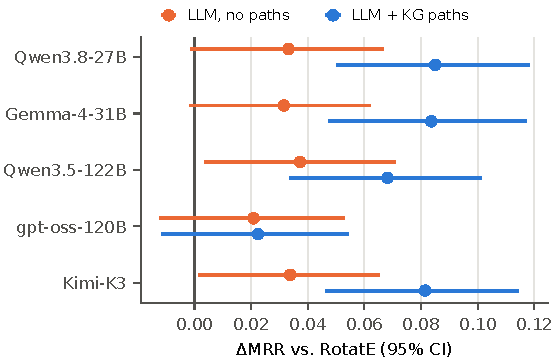
\includegraphics[width=0.62\textwidth]{figures/fig_accuracy.pdf}
\caption{Gain in MRR over RotatE (graph only, MRR 0.179) when each LLM re-ranks the RotatE top 20, without paths (orange) and with KG paths (blue). Whiskers: 95\% disease-level bootstrap CIs.\label{fig:accuracy}}
\end{figure}

\begin{table}[H]
\caption{RotatE test metrics over three training seeds (same split and hyper-parameters).\label{tab:seeds}}
\begin{tabularx}{\textwidth}{lcCCCC}
\toprule
\textbf{Seed} & \textbf{Best epoch} & \textbf{MRR} & \textbf{H@1} & \textbf{H@3} & \textbf{H@10}\\
\midrule
\tabinput{tables/kge_seeds.tex}
\bottomrule
\end{tabularx}
\end{table}

\subsection{Faithfulness}
Table~\ref{tab:faith} and Figure~\ref{fig:faith} report the judge's labels. Cited claims are almost always supported: 97--99\% are labelled \textsc{supported}, fewer than 0.5\% \textsc{unsupported}, and every cited path ID exists. The free-text mechanism is a different story: only 14--28\% of mechanism sentences are fully supported and 47--58\% are labelled \textsc{unsupported}. Inspection shows that mechanism sentences typically add a drug class, a mode of action or a clinical effect that is not in any path---true background knowledge, but not evidence from the graph. As a result only 4--18\% of explanations are supported in every statement.

Requiring each mechanism sentence to cite paths (prompt v2) changes this sharply (Table~\ref{tab:v2}): supported mechanism sentences rise from 28\% to 88\% (Qwen3.8-27B) and from 24\% to 91\% (Gemma-4-31B), and fully supported explanations from 16--18\% to 78--84\%. The models also write about half as many mechanism sentences. The cost is a small drop in accuracy on these 100 diseases ($-0.023$ and $-0.017$ MRR; the first CI just reaches zero, the second includes it) and a lower parse rate for Gemma-4-31B (97.1\%).

\TODO{Judge validation: Cohen's $\kappa$ between the judge and the first author's labels on 126 statements, overall and for mechanism sentences; note the error types observed (e.g.\ a direct indication claim labelled supported; honest ``the paths do not establish a mechanism'' sentences labelled unsupported).}

\begin{table}[H]
\caption{Faithfulness of grounded explanations (judge Nemotron-3-Super-120B; 100 test diseases, 20 candidates each). S/P/U: share of statements labelled supported / partial / unsupported. Pair all-S: share of explanations whose statements are all supported. Cite valid: share of claims whose cited IDs all exist.\label{tab:faith}}
\begin{adjustwidth}{-\extralength}{0cm}
\small
\begin{tabularx}{\fulllength}{lCCCCCCCCCC}
\toprule
\textbf{Model} & \textbf{Pairs} & \textbf{Stmts} & \textbf{Claim S} & \textbf{Claim U} & \textbf{Mech S} & \textbf{Mech P} & \textbf{Mech U} & \textbf{All S} & \textbf{Pair all-S} & \textbf{Cite valid}\\
\midrule
\tabinput{tables/faithfulness.tex}
\bottomrule
\end{tabularx}
\end{adjustwidth}
\end{table}

\begin{figure}[H]
\begin{adjustwidth}{-\extralength}{0cm}
\centering
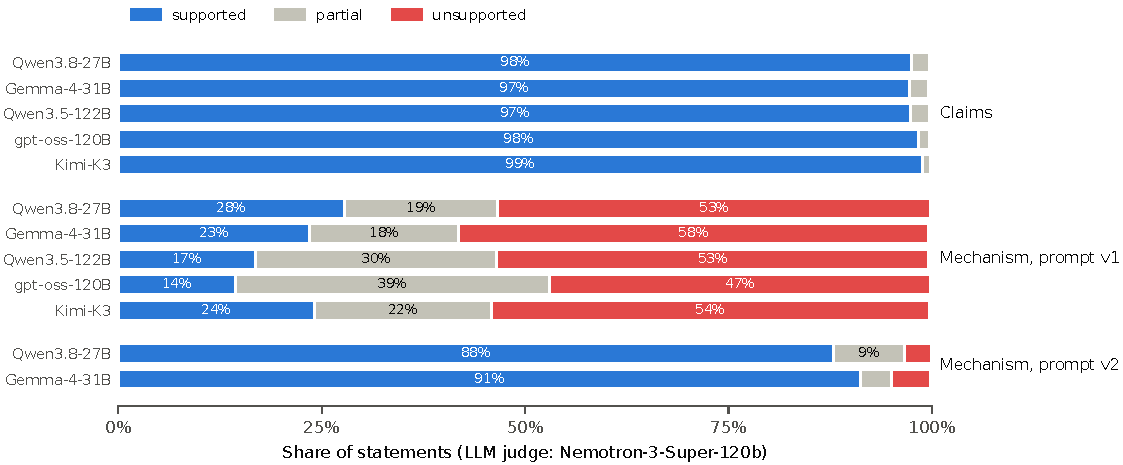
\includegraphics[width=0.9\linewidth]{figures/fig_faithfulness.pdf}
\end{adjustwidth}
\caption{Judge labels for cited claims, free-text mechanism sentences (prompt v1), and mechanism sentences that must cite paths (prompt v2, two models).\label{fig:faith}}
\end{figure}

\begin{table}[H]
\caption{Prompt v1 vs.\ v2 on the same 100 test diseases: accuracy and calibration (top), faithfulness (bottom). \dmrr{}: v2 minus v1 with 95\% disease-level bootstrap CI.\label{tab:v2}}
\begin{adjustwidth}{-\extralength}{0cm}
\small
\begin{tabularx}{\fulllength}{llCCCCCc}
\toprule
\textbf{Model} & \textbf{Prompt} & \textbf{MRR} & \textbf{H@1} & \textbf{H@10} & \textbf{ECE} & \textbf{AUROC} & \textbf{\dmrr{}}\\
\midrule
\tabinput{tables/prompt_v2_accuracy.tex}
\bottomrule
\end{tabularx}\\[4pt]
\begin{tabularx}{\fulllength}{lCCCCCCCCCC}
\toprule
\textbf{Model} & \textbf{Pairs} & \textbf{Stmts} & \textbf{Claim S} & \textbf{Claim U} & \textbf{Mech S} & \textbf{Mech P} & \textbf{Mech U} & \textbf{All S} & \textbf{Pair all-S} & \textbf{Cite valid}\\
\midrule
\tabinput{tables/prompt_v2_faithfulness.tex}
\bottomrule
\end{tabularx}
\end{adjustwidth}
\end{table}

\subsection{Calibration}
Raw confidences are badly over-confident (Table~\ref{tab:cal}, Figure~\ref{fig:cal}a): the mean confidence of grounded models is 0.27--0.33 while only 3.5\% of candidates are held-out indications, giving ECE 0.24--0.29. The confidences nevertheless \emph{rank} well: AUROC is 0.80--0.90 (Kimi-K3 0.902), and grounding raises AUROC over the no-paths baseline for four of five models, matching the accuracy results. The problem is therefore a scale offset rather than a lack of signal.

Post-hoc maps fitted on 100 validation diseases confirm this (Table~\ref{tab:recal}, Figure~\ref{fig:cal}b). Temperature scaling, which cannot move a confidence of 0.5 and so cannot correct a base-rate offset, helps little (ECE 0.13--0.28). Platt scaling, which adds a bias term, reduces test ECE to 0.005--0.013 and the Brier score to about 0.03 for every model; isotonic regression performs similarly. Because nearly all recalibrated confidences fall in the lowest equal-width bin, that ECE could flatter these maps; ECE with ten equal-count bins confirms the result (0.005--0.009 after Platt scaling, vs.\ 0.24--0.29 raw), as does the Brier score, which does not depend on binning.

\begin{table}[H]
\caption{Calibration of LLM confidence over all test disease--candidate pairs (base rate 0.035). Parse: share of parsable responses.\label{tab:cal}}
\begin{tabularx}{\textwidth}{llCCCCC}
\toprule
\textbf{Model} & \textbf{Mode} & \textbf{Parse} & \textbf{Mean conf.} & \textbf{ECE} & \textbf{Brier} & \textbf{AUROC}\\
\midrule
\tabinput{tables/calibration.tex}
\bottomrule
\end{tabularx}
\end{table}

\begin{table}[H]
\caption{Test calibration of grounded confidences after maps fitted on 100 validation diseases. ECE: ten equal-width bins; ECE-m: ten equal-count bins. Maps are monotone, so accuracy is unchanged.\label{tab:recal}}
\begin{adjustwidth}{-\extralength}{0cm}
\small
\begin{tabularx}{\fulllength}{llcCCCCC}
\toprule
\textbf{Model} & \textbf{Map} & \textbf{Parameters} & \textbf{Mean conf.} & \textbf{ECE} & \textbf{ECE-m} & \textbf{Brier} & \textbf{AUROC}\\
\midrule
\tabinput{tables/recalibration.tex}
\bottomrule
\end{tabularx}
\end{adjustwidth}
\end{table}

\begin{figure}[H]
\begin{adjustwidth}{-\extralength}{0cm}
\centering
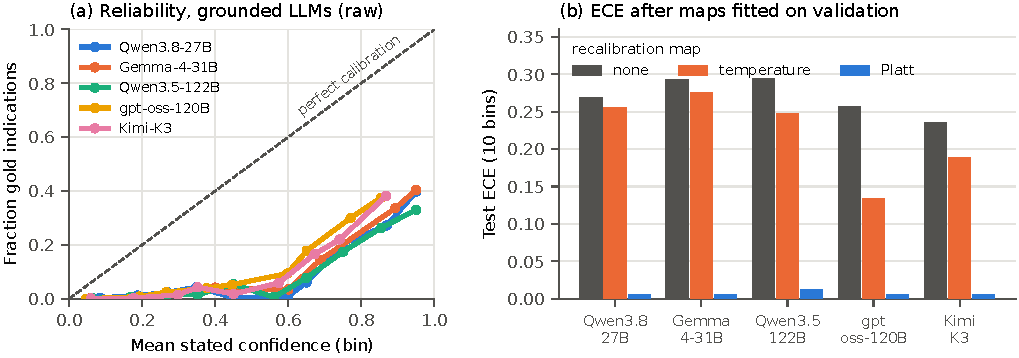
\includegraphics[width=0.95\linewidth]{figures/fig_calibration.pdf}
\end{adjustwidth}
\caption{(\textbf{a}) Reliability of raw grounded confidences (bins with at least 30 pairs); all models lie far below the diagonal. (\textbf{b}) Test ECE before and after temperature and Platt maps fitted on validation diseases.\label{fig:cal}}
\end{figure}

\subsection{Robustness to KG Poisoning}
\textbf{Training-time poisoning} barely affects RotatE (Table~\ref{tab:rob_kge}): MRR is unchanged (0.179 vs.\ 0.183 targeted, 0.192 random), and the targeted attack doubles the share of diseases where the decoy is ranked first (5.0\% to 10.3\%) without changing the decoy's median rank.

\textbf{Retrieval-time poisoning} is far more effective against the grounded LLMs (Table~\ref{tab:rob_llm}, Figure~\ref{fig:poison}). Three fake chains per decoy raise the share of diseases where the decoy is ranked first from 4--5\% to 9--20\% and halve its median rank (from 11--12 to 4--6); the decoy rises in rank for 62--73\% of diseases, and its mean confidence rises by 0.10--0.22. In 98.6--100\% of decoy explanations the LLM cites the fake edges: the explanation is faithful to the graph, but the graph is wrong. Accuracy on the true indications drops only slightly ($\le0.02$ MRR), so the attack would be invisible in aggregate metrics. gpt-oss-120B and Gemma-4-31B are the most susceptible (19.8\% and 19.4\% decoy at rank 1), Qwen3.5-122B the least (9.3\%). Random poisoning at 5\% has no measurable effect (Table~\ref{tab:rob_rand}): only 2.4\% of explanations contain a fake path, and MRR changes by at most 0.003.

\begin{figure}[H]
\centering
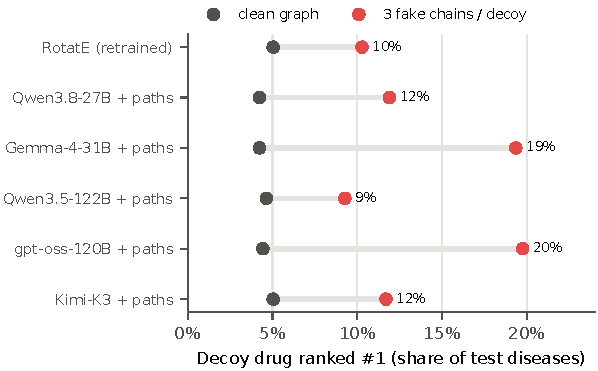
\includegraphics[width=0.62\textwidth]{figures/fig_poisoning.pdf}
\caption{Share of test diseases where the decoy drug is ranked first, on the clean graph and after injecting three fake chains per decoy. RotatE is retrained on the poisoned graph; the LLMs re-rank clean RotatE candidates with paths retrieved from the poisoned graph.\label{fig:poison}}
\end{figure}

\begin{table}[H]
\caption{Training-time poisoning: RotatE retrained on the poisoned graph. Decoy@1: share of diseases where the decoy is ranked first; Decoy med: its median rank (clean $\to$ poisoned).\label{tab:rob_kge}}
\begin{tabularx}{\textwidth}{lCCCCC}
\toprule
\textbf{Graph} & \textbf{MRR} & \textbf{H@1} & \textbf{H@10} & \textbf{Decoy@1} & \textbf{Decoy med}\\
\midrule
\tabinput{tables/robustness_kge.tex}
\bottomrule
\end{tabularx}
\end{table}

\begin{table}[H]
\caption{Retrieval-time targeted poisoning (clean $\to$ poisoned). Promoted: share of diseases where the decoy moves up. Cites fake: share of decoy explanations whose claims cite a fake edge. Gold MRR: accuracy on true indications.\label{tab:rob_llm}}
\begin{adjustwidth}{-\extralength}{0cm}
\small
\begin{tabularx}{\fulllength}{lCCCCCC}
\toprule
\textbf{Model} & \textbf{Decoy@1} & \textbf{Decoy med} & \textbf{Decoy conf.} & \textbf{Promoted} & \textbf{Cites fake} & \textbf{Gold MRR}\\
\midrule
\tabinput{tables/robustness_llm_targeted.tex}
\bottomrule
\end{tabularx}
\end{adjustwidth}
\end{table}

\begin{table}[H]
\caption{Retrieval-time random poisoning (5\% fake drug--protein and disease--protein edges), on pairs whose retrieved paths changed. With fake: share of explanations shown a fake path; Cites fake: share citing one.\label{tab:rob_rand}}
\begin{tabularx}{\textwidth}{lCCCCC}
\toprule
\textbf{Model} & \textbf{Pairs} & \textbf{Gold MRR} & \textbf{Gold H@1} & \textbf{With fake} & \textbf{Cites fake}\\
\midrule
\tabinput{tables/robustness_llm_random.tex}
\bottomrule
\end{tabularx}
\end{table}

\subsection{Disease-Held-Out Split}\label{sec:zeroshot}
Table~\ref{tab:disease} repeats the accuracy comparison on the disease-held-out split, where the KG contains no indication, contraindication or off-label edge for any test disease. The same pipeline is retrained end to end: RotatE and TxGNN on the new training graph, path retrieval on that graph, and all five LLMs with and without paths on the new RotatE top 20 (2,720 pairs per model and mode). We verified that no retrieved path contains an edge between a drug and a held-out disease.

The task is harder for the graph models: RotatE drops to MRR 0.109 (random split: 0.179) and only 24.3\% of gold drugs reach its top 20. TxGNN, although designed for diseases without known treatments, does not overtake RotatE in our protocol (MRR 0.040, Hits@10 0.102; 13.5\% of gold drugs in its top 20), so the ranking gap seen on the random split persists.

LLM re-ranking helps more here than on the random split in relative terms. All five grounded LLMs improve on RotatE (\dmrr{} $+0.039$ to $+0.082$, all CIs above zero), and for four of them the paths add a significant $+0.034$ to $+0.054$ MRR over the same model without paths; gpt-oss-120B again gains nothing from the paths ($+0.006$ [$-0.015$, $+0.025$]), consistent with Section~\ref{sec:accuracy}. Without paths the LLMs gain only $+0.023$ to $+0.041$, and in this setting a no-paths gain can come only from the LLM's prior knowledge, not from the graph. Grounded confidences also separate gold from non-gold candidates better than on the random split (AUROC 0.93--0.96 vs.\ 0.86--0.91 without paths; Table~\ref{tab:disease_cal}), but they remain over-confident (ECE 0.10--0.15).

\textbf{Where the zero-shot evidence comes from.} With treatment edges removed, the most informative paths are analogies: the candidate is indicated for (or used off-label for) a disease that is linked to the target disease by a parent/child ontology edge. Such a path exists for 99.5\% of the gold pairs in the top 20 that have any path, and for 40.6\% of the non-gold pairs. The LLMs therefore mostly transfer indications from neighbouring diseases in the ontology. This is a legitimate and interpretable signal for an unseen disease---and the explanation names the related disease---but it means that this split measures transfer to diseases that have treated relatives, not repurposing for diseases with no treated neighbours.

\begin{table}[H]
\caption{Accuracy on the disease-held-out split (876 indications of 136 test diseases with no drug--disease edges in training). LLM rows re-rank the RotatE top 20; \dmrr{} columns as in Table~\ref{tab:accuracy}.\label{tab:disease}}
\begin{adjustwidth}{-\extralength}{0cm}
\small
\begin{tabularx}{\fulllength}{lcccCC}
\toprule
\textbf{Method} & \textbf{MRR} & \textbf{H@1} & \textbf{H@10} & \textbf{\dmrr{} vs.\ RotatE} & \textbf{\dmrr{} vs.\ no paths}\\
\midrule
\tabinput{tables/disease_accuracy.tex}
\bottomrule
\end{tabularx}
\end{adjustwidth}
\end{table}

\begin{table}[H]
\caption{Calibration of LLM confidence on the disease-held-out split (all 2,720 pairs per model and mode; raw confidences, no recalibration).\label{tab:disease_cal}}
\begin{tabularx}{\textwidth}{llCCCC}
\toprule
\textbf{Model} & \textbf{Mode} & \textbf{Parse rate} & \textbf{Mean conf.} & \textbf{ECE} & \textbf{AUROC}\\
\midrule
\tabinput{tables/disease_calibration.tex}
\bottomrule
\end{tabularx}
\end{table}

%======================================================================
\section{Discussion}
%======================================================================
\textbf{Grounding helps accuracy, but not for every model.} Four of five LLMs gain significantly from the paths beyond what they gain from names alone, which indicates that they use the graph evidence rather than only their prior. gpt-oss-120B does not, although its explanations are equally well cited, which shows that following the citation format and using the evidence for the decision are separate abilities. Model size is not the deciding factor: a 27B dense model matches the largest MoE model.

\textbf{Citations are faithful; prose is not, unless forced.} Measuring faithfulness at the level of cited claims alone would suggest near-perfect grounding. The free-text mechanism---the part a human is most likely to read---mostly contains material from outside the paths. Requiring a citation per sentence nearly closes this gap at a small accuracy cost, so we recommend sentence-level citation for any user-facing explanation, and recommend that faithfulness evaluations score all generated text, not only the parts that carry citations.

\textbf{Confidence is useful after recalibration.} LLM confidences carry real ranking signal but should not be shown to users as probabilities. A two-parameter Platt map fitted on a few hundred validation pairs is enough to make them calibrated for this task.

\textbf{Grounding moves trust to the graph.} The poisoning results show the other side of faithfulness: a grounded LLM is only as reliable as its evidence. A few planted edges promote a decoy with a well-cited explanation, and aggregate accuracy hides the attack. Provenance logging makes such failures traceable---every cited path can be traced to its source edge---but does not prevent them. Practical defences include checking cited edges against source databases, flagging candidates whose support rests on few recently added edges, and monitoring decoy-style rank changes.

\textbf{Limitations.} (i) \emph{Memorisation.} Most test indications are approved uses that the LLMs have likely seen during training~\cite{carlini2021extracting}. The no-paths baseline estimates this effect (+0.02--0.04 MRR over RotatE); the grounding gain is measured on top of it, but absolute LLM accuracy on truly novel repurposing hypotheses may be lower. The disease-held-out split removes the answer from the graph but not from LLM pre-training; there the no-paths gain (+0.02--0.04) bounds the prior-knowledge effect. (ii) \emph{LLM judge.} Faithfulness labels come from one LLM judge, which errs in both directions; we validate it against a single annotator on 126 statements. (iii) \emph{Re-ranking ceiling.} Only 37.7\% of gold drugs are in the RotatE top 20, so re-ranking cannot help the rest. (iv) \emph{Single graph and split.} Results are for one KG and one random split (plus the disease-held-out split); LLM results use one RotatE seed, and two of three RotatE seeds were still improving at the 50-epoch limit. (v) \emph{TxGNN} was run with a larger pre-training batch than published and one seed, on CPU. (vi) Prompt v2 was tested on two models and 100 diseases. (vii) \emph{Disease split.} Held-out diseases keep their ontology edges, and many have closely related treated diseases; the zero-shot gains rely largely on these neighbours (Section~\ref{sec:zeroshot}), so a split that withholds whole disease areas~\cite{huang2024txgnn} would be harder.

%======================================================================
\section{Conclusions}
%======================================================================
We framed drug repurposing as a KG-grounded recommendation task and evaluated not only accuracy but faithfulness, calibration and robustness across five LLMs. Grounded LLM re-ranking improves a strong KG-embedding recommender, and the paths themselves contribute to the gain, also for diseases with no treatment edges in the graph, where the evidence is mostly the indications of related diseases. Explanations are faithful when every sentence must cite evidence, and confidences become calibrated with a simple validation-fitted map. The same grounding, however, allows a handful of planted edges to promote a decoy with a convincing, well-cited explanation. Trustworthy repurposing recommenders therefore need sentence-level citation, recalibrated confidence, full provenance and checks on the integrity of the graph itself.

\vspace{6pt}

\authorcontributions{Conceptualization, K.N.; methodology, K.N. and H.J.; software, K.N.; validation, K.N.; formal analysis, K.N.; investigation, K.N.; data curation, K.N.; visualization, K.N.; writing---original draft preparation, K.N.; writing---review and editing, H.J. and K.N.; supervision, H.J. All authors have read and agreed to the published version of the manuscript.}

% AUTHOR CONFIRMATION REQUIRED: grants copied from the RAGO/RAMP/PROBE manuscripts; confirm they apply to this study.
\funding{This research was supported in part by the National Institutes of Health IDeA grant P20GM103408, the National Science Foundation CSSI grant OAC 2410668, and the USDA-NIFA Sustainable Agriculture Systems grant 2020-69012-31871.}

\institutionalreview{Not applicable.}

\informedconsent{Not applicable.}

\dataavailability{PrimeKG v2.1 is available from Harvard Dataverse (\url{https://doi.org/10.7910/DVN/IXA7BM}). Code, prompts, split definitions and provenance logs are available in the GitHub repository \url{https://github.com/utpoln/trustworthy-drug-repurposing} \TODO{archive DOI (e.g.\ Zenodo) for the submitted version}.}

% AUTHOR CONFIRMATION REQUIRED: the GenAI statement must match how the AI assistant was actually used.
\acknowledgments{The authors thank the University of Idaho Research Computing team for access to the MindRouter API gateway~\cite{sheneman2026mindrouter} used for all model inference in this study. Separately from the LLMs evaluated in this study, during its preparation the authors used Claude (Anthropic; Claude Opus 5.5) through the Claude Code environment as an AI assistant. It wrote and executed code for the data splits, candidate generation, path retrieval, LLM and judge runs, poisoning experiments and statistical analysis; drafted manuscript text, tables, figure code and bibliography entries; and drafted labels for the judge-validation sample. The authors defined the study's aims and design, reviewed each design decision, and checked the code, results, references and text. The authors take full responsibility for the content of this publication.}

\conflictsofinterest{The authors declare no conflicts of interest.}

\abbreviations{Abbreviations}{
The following abbreviations are used in this manuscript:
\\
\noindent
\begin{tabular}{@{}ll}
AUROC & Area under the receiver operating characteristic curve\\
CI & Confidence interval\\
ECE & Expected calibration error\\
KG & Knowledge graph\\
LLM & Large language model\\
MoE & Mixture of experts\\
MRR & Mean reciprocal rank\\
RRF & Reciprocal rank fusion
\end{tabular}
}

\appendixtitles{yes}
\appendixstart
\appendix
\section{Prompts}\label{app:prompts}
All prompts are reproduced verbatim below (long lines wrapped for print; wrapped continuation lines are indented). Placeholders in braces are filled per request; in the user prompt, \texttt{\{paths\}} is the numbered list \texttt{P1: \ldots}, \texttt{P2: \ldots} of path texts, and in the judge prompt each statement is followed by its cited path IDs or \texttt{[cites: none]}. The template version is recorded in every provenance record. Source: \texttt{src/llm/prompts.py} and \texttt{src/eval/faithfulness.py}.

% generated by experiments/make_prompt_appendix.py -- do not edit
\paragraph{Grounded system prompt, grounded-v1 (main experiments).}
{\footnotesize
\begin{verbatim}
You are a biomedical knowledge-graph analyst assessing drug repurposing candidates.

Rules:
1. Use ONLY the knowledge-graph paths given by the user. Do not use any outside knowledge,
  even if you believe it is true. If the paths do not support a mechanism, say so.
2. Every claim must cite the IDs of the paths that support it (e.g. ["P1", "P4"]). A claim
  may only state relations that appear in its cited paths.
3. Judge how strongly the paths, taken together, support the drug as a treatment for the
  disease. Paths through drug-metabolising enzymes, carriers or transporters, or through
  very general disease categories, are weak evidence of therapeutic effect.
4. Give a confidence in [0, 1] that the drug is an effective treatment (indication) for the
  disease, based only on the paths. Be calibrated: 0.5 means a coin flip.

Respond with a single JSON object and nothing else:
{
  "claims": [{"text": "<one sentence>", "paths": ["P1"]}],
  "mechanism": "<2-4 sentence explanation built only from the claims>",
  "evidence_strength": "strong" | "moderate" | "weak" | "none",
  "confidence": <number between 0 and 1>
}
\end{verbatim}
}

\paragraph{Grounded user prompt (both versions).}
{\footnotesize
\begin{verbatim}
Disease: {disease}
Candidate drug: {drug}

Knowledge-graph paths linking the drug to the disease (arrows show edge direction; -[ ]-
  means the relation is symmetric):
{paths}

Assess whether {drug} could treat {disease}, using only these paths.
\end{verbatim}
}

\paragraph{Grounded system prompt, grounded-v2 (forced-citation experiment); differences from v1 are in rule 3 and the mechanism field.}
{\footnotesize
\begin{verbatim}
You are a biomedical knowledge-graph analyst assessing drug repurposing candidates.

Rules:
1. Use ONLY the knowledge-graph paths given by the user. Do not use any outside knowledge,
  even if you believe it is true.
2. Every claim must cite the IDs of the paths that support it (e.g. ["P1", "P4"]). A claim
  may only state relations that appear in its cited paths.
3. The mechanism is a list of 2-4 sentences. EVERY mechanism sentence must cite the paths it
  is built from, and may only combine relations that appear in those paths. Do not name any
  biological process, pathway, drug class or effect that is not written in a cited path. If
  the paths do not show a therapeutic mechanism, write one sentence saying which kinds of
  relation the paths contain (citing them) and that they do not establish a mechanism.
4. Judge how strongly the paths, taken together, support the drug as a treatment for the
  disease. Paths through drug-metabolising enzymes, carriers or transporters, or through
  very general disease categories, are weak evidence of therapeutic effect.
5. Give a confidence in [0, 1] that the drug is an effective treatment (indication) for the
  disease, based only on the paths. Be calibrated: 0.5 means a coin flip.

Respond with a single JSON object and nothing else:
{
  "claims": [{"text": "<one sentence>", "paths": ["P1"]}],
  "mechanism": [{"text": "<one sentence>", "paths": ["P1", "P2"]}],
  "evidence_strength": "strong" | "moderate" | "weak" | "none",
  "confidence": <number between 0 and 1>
}
\end{verbatim}
}

\paragraph{No-paths system and user prompts (no-paths-v1).}
{\footnotesize
\begin{verbatim}
You are a biomedical expert assessing drug repurposing candidates.

Give a confidence in [0, 1] that the drug is an effective treatment (indication) for the
  disease. Be calibrated: 0.5 means a coin flip.

Respond with a single JSON object and nothing else:
{
  "mechanism": "<2-4 sentence explanation>",
  "confidence": <number between 0 and 1>
}

Disease: {disease}
Candidate drug: {drug}

Could {drug} treat {disease}?
\end{verbatim}
}

\paragraph{Faithfulness judge system and user prompts (judge-v1, judge Nemotron-3-Super-120b).}
{\footnotesize
\begin{verbatim}
You check whether statements are supported by knowledge-graph paths.

For each statement, decide using ONLY the listed paths (for statements with cited paths,
  only those cited paths; for statements with no citations, any of the paths):
- "SUPPORTED": every fact in the statement is stated by the paths. Restating a path in other
  words is fine. Calling a chain of relations an association or link is fine.
- "PARTIAL": some facts are in the paths, but the statement adds a fact that is not (for
  example a drug class, a mode of action, a biological effect, or a clinical claim).
- "UNSUPPORTED": the main fact is not in the paths, or contradicts them.
Do not use your own biomedical knowledge to fill gaps: a true fact that is not in the paths
  is NOT supported.

Respond with a single JSON object and nothing else:
{"labels": [{"id": "S1", "label": "SUPPORTED" | "PARTIAL" | "UNSUPPORTED", "reason":
  "<short>"}]}

Paths:
{paths}

Statements:
{statements}
\end{verbatim}
}


\begin{adjustwidth}{-\extralength}{0cm}
\reftitle{References}
\bibliography{references}
\end{adjustwidth}
\end{document}
